\documentclass[a4paper,12pt]{article}
\usepackage[utf8]{inputenc}
\usepackage[margin=1in]{geometry}
\usepackage{enumitem}
\usepackage{xcolor}
\usepackage{titlesec}
\usepackage{tcolorbox}
\usepackage{fancyhdr}
\usepackage{graphicx}
\usepackage{tikz}
\usetikzlibrary{shapes,arrows,positioning,fit,calc}

% Color scheme - professional blues and accents
\definecolor{primaryblue}{RGB}{211, 11, 10}
\definecolor{accentblue}{RGB}{200, 140, 100}
\definecolor{lightblue}{RGB}{234, 214, 142}
\definecolor{darkgray}{RGB}{52, 73, 94}
\definecolor{lightgray}{RGB}{236, 240, 241}
\definecolor{accentorange}{RGB}{200, 100, 100}

% Configure tcolorbox
\tcbuselibrary{skins,breakable}

% Title formatting
\titleformat{\section}
  {\Large\bfseries\color{primaryblue}}
  {\thesection}{1em}{}
  [\titlerule]

\titleformat{\subsection}
  {\large\bfseries\color{accentblue}}
  {\thesubsection}{1em}{}

\titleformat{\paragraph}[hang]
  {\normalfont\bfseries\color{darkgray}}
  {}{0em}{}

% Header and footer
\pagestyle{fancy}
\fancyhf{}
\fancyhead[L]{\color{primaryblue}\small CS2323 Computer Architecture}
\fancyhead[R]{\color{accentblue}\small Coreographer}
\fancyfoot[C]{\color{darkgray}\thepage}
\renewcommand{\headrulewidth}{0.5pt}
\renewcommand{\footrulewidth}{0pt}
\renewcommand{\headrule}{\hbox to\headwidth{\color{accentblue}\leaders\hrule height \headrulewidth\hfill}}

% Custom title
\title{
  \vspace{-1.5cm}
  \begin{tcolorbox}[
    colback=primaryblue,
    colframe=primaryblue,
    arc=3mm,
    boxrule=0pt,
    left=10pt,
    right=10pt,
    top=15pt,
    bottom=15pt
  ]
  \color{white}
  \LARGE\bfseries Coreographer \\[0.2em]
  \large Micro-task Scheduled Multi-core RISC-V Architecture \\[0.1em]
  \normalsize Revised Scope Document
  \end{tcolorbox}
  \vspace{-0.5cm}
}

\author{
  \begin{tcolorbox}[
    colback=lightgray,
    colframe=lightgray,
    arc=2mm,
    boxrule=0pt,
    left=8pt,
    right=8pt,
    top=8pt,
    bottom=8pt
  ]
  \color{darkgray}
  \textbf{E. Mihir Divyansh} \\ 
  \small EE23BTECH11017
  \end{tcolorbox}
}
\date{}

\begin{document}
\maketitle
\thispagestyle{fancy}

\section*{Executive Summary}

\begin{tcolorbox}[
  colback=lightblue!30,
  colframe=accentblue,
  arc=2mm,
  boxrule=1.5pt,
  left=10pt,
  right=10pt,
  top=10pt,
  bottom=10pt
]
This project implements a \textbf{heterogeneous multi-core RISC-V architecture} inspired by GPU streaming multiprocessors, featuring clustered cores with local register sharing and a hardware-based micro-task scheduler. The design targets moderately parallel workloads where task-level parallelism can be exploited without the overhead of a full OS.
\end{tcolorbox}

\section*{Architecture Overview}

\begin{enumerate}[leftmargin=*, itemsep=0.3em]
    \item \textbf{\color{accentorange}Neighbor-based register sharing} replaces global shared register file
    \begin{itemize}
        \item Each core has its own private 32-register file (RV32I standard)
        \item Cores can access registers from neighboring cores via extended instructions
        \item Neighbor topology is configurable (And is optionally a performance affecting parameter)
        \item \textbf{Exploration aspect: (Optional)} Different topologies can be implemented and compared
    \end{itemize}   
    
    \item \textbf{\color{accentorange}Parallel hardware scheduler} as dedicated dispatch unit
    \begin{itemize}
        \item Maintains instruction cache and ready queue for worker cores
        \item Broadcasts tasks on shared dispatch bus
        \item Cores pull tasks when available
    \end{itemize}
    
    \item \textbf{\color{accentorange}Micro-task programming model}
    \begin{itemize}
        \item Input programs structured as self-contained micro-tasks. (To be defined)
        \item Tasks declare dependencies and resource requirements in headers 
    \end{itemize}
\end{enumerate}

\subsection*{System Block Diagram}

\begin{figure}
\begin{center}
  \scalebox{0.7}
{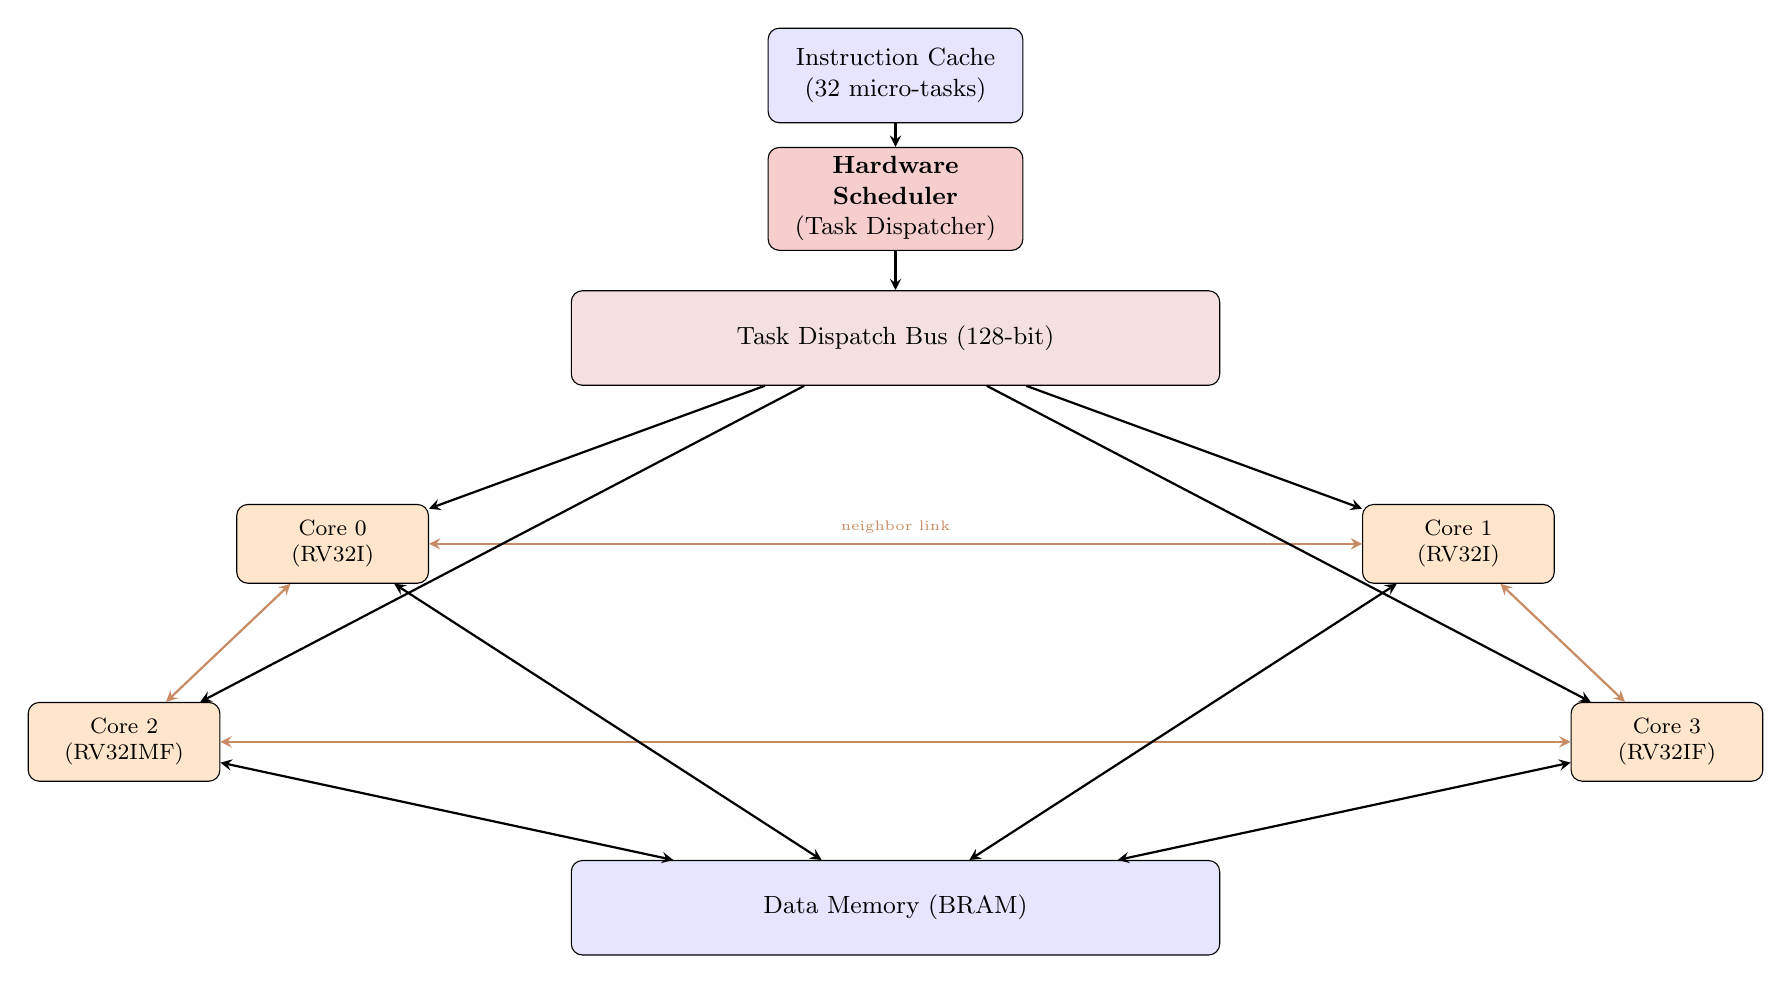
\begin{tikzpicture}[
    scale = 0.8,
    node distance=0.3cm and 0.5cm,
    block/.style={rectangle, draw, fill=blue!10, text width=3cm, text centered, rounded corners, minimum height=1.2cm, font=\small},
    core/.style={rectangle, draw, fill=orange!20, text width=2.2cm, text centered, rounded corners, minimum height=1cm, font=\footnotesize},
    reg/.style={rectangle, draw, fill=yellow!30, text width=2cm, text centered, minimum height=0.6cm, font=\footnotesize},
    arrow/.style={->, >=stealth, thick},
    bidir/.style={<->, >=stealth, thick, color=accentblue}
]

% Scheduler block
\node[block, fill=primaryblue!20] (scheduler) at (0,3) {\textbf{Hardware Scheduler}\\(Task Dispatcher)};
\node[block, above=0.3cm of scheduler] (icache) {Instruction Cache\\(32 micro-tasks)};

% Dispatch bus
\node[block, fill=accentorange!20, below=0.5cm of scheduler, text width=8cm] (bus) {Task Dispatch Bus (128-bit)};

% Core arrangement in ring topology (example)
\node[core, below left=1.5cm and 1.8cm of bus] (core0) {Core 0\\(RV32I)};
\node[core, below right=1.5cm and 1.8cm of bus] (core1) {Core 1\\(RV32I)};
\node[core, below left=1.5cm and 0.2cm of core0] (core2) {Core 2\\(RV32IMF)};
\node[core, below right=1.5cm and 0.2cm of core1] (core3) {Core 3\\(RV32IF)};

% Neighbor connections (ring topology shown)
\draw[bidir] (core0) -- (core1) node[midway, above, font=\tiny] {neighbor link};
\draw[bidir] (core1) -- (core3);
\draw[bidir] (core3) -- (core2);
\draw[bidir] (core2) -- (core0);

% Memory system
\node[block, below=1.5cm of $(core2)!0.5!(core3)$, text width=8cm] (mem) {Data Memory (BRAM)};

% Arrows from bus to cores
\draw[arrow] (icache) -- (scheduler);
\draw[arrow] (scheduler) -- (bus);
\draw[arrow] (bus) -- (core0);
\draw[arrow] (bus) -- (core1);
\draw[arrow] (bus) -- (core2);
\draw[arrow] (bus) -- (core3);

% Memory connections
\draw[arrow, <->] (core0) -- (mem);
\draw[arrow, <->] (core1) -- (mem);
\draw[arrow, <->] (core2) -- (mem);
\draw[arrow, <->] (core3) -- (mem);

\end{tikzpicture}}
\caption{Example Block Diagram of System}
\end{center}
\end{figure}
\vspace{0.3cm}
\begin{tcolorbox}[
  colback=lightblue!20,
  colframe=accentblue,
  arc=2mm,
  boxrule=1pt,
  left=8pt,
  right=8pt,
  top=5pt,
  bottom=5pt
]

One topology will be chosen for initial implementation, with potential to compare alternatives in stretch goals.
\end{tcolorbox}


\section*{Micro-Task Format}

Each micro-task consists of a \textbf{header} (metadata) and a \textbf{body} (instructions).

\paragraph{Task Header Format (32 bits):}
\begin{verbatim}
[31:24] Task ID (8 bits)
[23:16] Dependency vector (8 bits) - IDs of prerequisite tasks
[15:12] Capability flags (4 bits):
        bit 3: Requires multiply (→ must go to Cluster 1)
        bit 2: Requires division
        bit 1: Memory-intensive (hint)
        bit 0: Reserved
[11:8]  Cluster preference (4 bits): 0=any, 1=Cluster0, 2=Cluster1
[7:0]   Instruction count (8 bits): number of instructions in body
\end{verbatim}

\paragraph{Task Body:} 
\begin{itemize}
    \item Sequence of 4-16 standard RV32I(M) instructions
    \item Last instruction must be task completion marker (custom: \texttt{TASK\_DONE})
    \item No branches outside task boundary (tasks are atomic)
    \item Example:
\end{itemize}

\begin{tcolorbox}[
  colback=lightgray!50,
  colframe=darkgray,
  arc=1mm,
  boxrule=0.5pt,
  left=5pt,
  right=5pt,
  top=5pt,
  bottom=5pt,
  fontupper=\ttfamily\footnotesize
]
.task 42 \# Task ID\\
.depends 39, 40 \# Wait for tasks 39 and 40\\
.needs\_mul \# Requires Cluster 1\\
.instructions\\
\hspace{1em}lw   r1, 0(r10)  \# Load A[i]\\
\hspace{1em}lw   r2, 0(r11)  \# Load B[i]\\
\hspace{1em}mul  r3, r1, r2  \# Multiply\\
\hspace{1em}sw   r3, 0(r12)  \# Store C[i]\\
\hspace{1em}TASK\_DONE       \# Signal completion\\
.end\_task
\end{tcolorbox}

\section*{Benchmark Selection}

\begin{tcolorbox}[
  colback=lightblue!20,
  colframe=accentblue,
  arc=2mm,
  boxrule=1pt,
  left=8pt,
  right=8pt,
  top=8pt,
  bottom=8pt,
  breakable
]
\textbf{Selection Criteria:}
\begin{itemize}
    \item Exhibit moderate task-level parallelism (not embarrassingly parallel)
    \item Fit in on-chip memory (32 KB data limit) (Optionally stream from host)
    \item Simple enough to manually decompose into micro-tasks
    \item Demonstrate heterogeneous core utilization
\end{itemize}
\end{tcolorbox}

\paragraph{Benchmark 1: Vector Dot Product}
\begin{itemize}
    \item \textbf{Size:} Two 64-element vectors (512 bytes total)
    \item \textbf{Why:} Simple, verifiable, demonstrates basic dispatch.
    \item \textbf{Task decomposition:} Each task computes one element: \texttt{result[i] = A[i] * B[i]}
\end{itemize}

\paragraph{Benchmark 2: Small Dense Matrix Multiply}
\begin{itemize}
    \item \textbf{Size:} 8$\times$8 or 16$\times$16 matrices (depending on memory constraints)
    \item \textbf{Task decomposition:} Each task computes one output element via dot product
\end{itemize}

\paragraph{Benchmark 3: Streaming Accumulator}
\begin{itemize}
    \item \textbf{Size:} 256-element stream, 8-tap accumulator window
    \item \textbf{Parallelism:} Pipeline with overlapping windows
    \item \textbf{Why:} Tests scheduler's ability to maintain steady-state throughput
\end{itemize}

\section*{Evaluation Metrics}

\subsection*{Performance Metrics}
\begin{itemize}
    \item \textbf{Throughput}
    \item \textbf{Speedup} 
    \item \textbf{Core utilization:} \% of cycles each core is executing instructions
    \item \textbf{Scheduler efficiency:} Dispatch stalls / total dispatch attempts
    \item \textbf{CPI per core}
    \item \textbf{Neighbor access metrics:}
    \begin{itemize}
        \item Neighbor register read/write counts per core
        \item Average latency per neighbor access
        \item Neighbor access efficiency (successful / attempted)
    \end{itemize}
\end{itemize}

\subsection*{Resource Utilization}
\begin{itemize}
    \item LUT count, BRAM, DSP usage
    \item Maximum clock frequency
    \item Power consumption estimate
\end{itemize}

\subsection*{Scope of Future Work}
\begin{itemize}
    \item Topology comparison: Topology vs performance on different workloads.
    \item Vary core count (2, 4, 8 cores) to study neighbor network scaling
    \item Compare homogeneous (all RV32I) vs heterogeneous (RV32I + RV32IM) configurations
    \item Analyze neighbor access latency sensitivity (1-cycle vs 2-cycle access times)
\end{itemize}

\section*{Deliverables}

\begin{enumerate}[leftmargin=*]
    \item \textbf{RTL codebase:} Synthesizable Verilog/VHDL for all system components
    \item \textbf{Benchmark Results:} At least 2 working micro-task programs with verification datasets
    \item \textbf{FPGA demonstration:} Live demo showing parallel execution and performance counters
\end{enumerate}
\end{document}